\documentclass{standalone}
\usepackage{tikz}
\usetikzlibrary{patterns, positioning}

\begin{document}
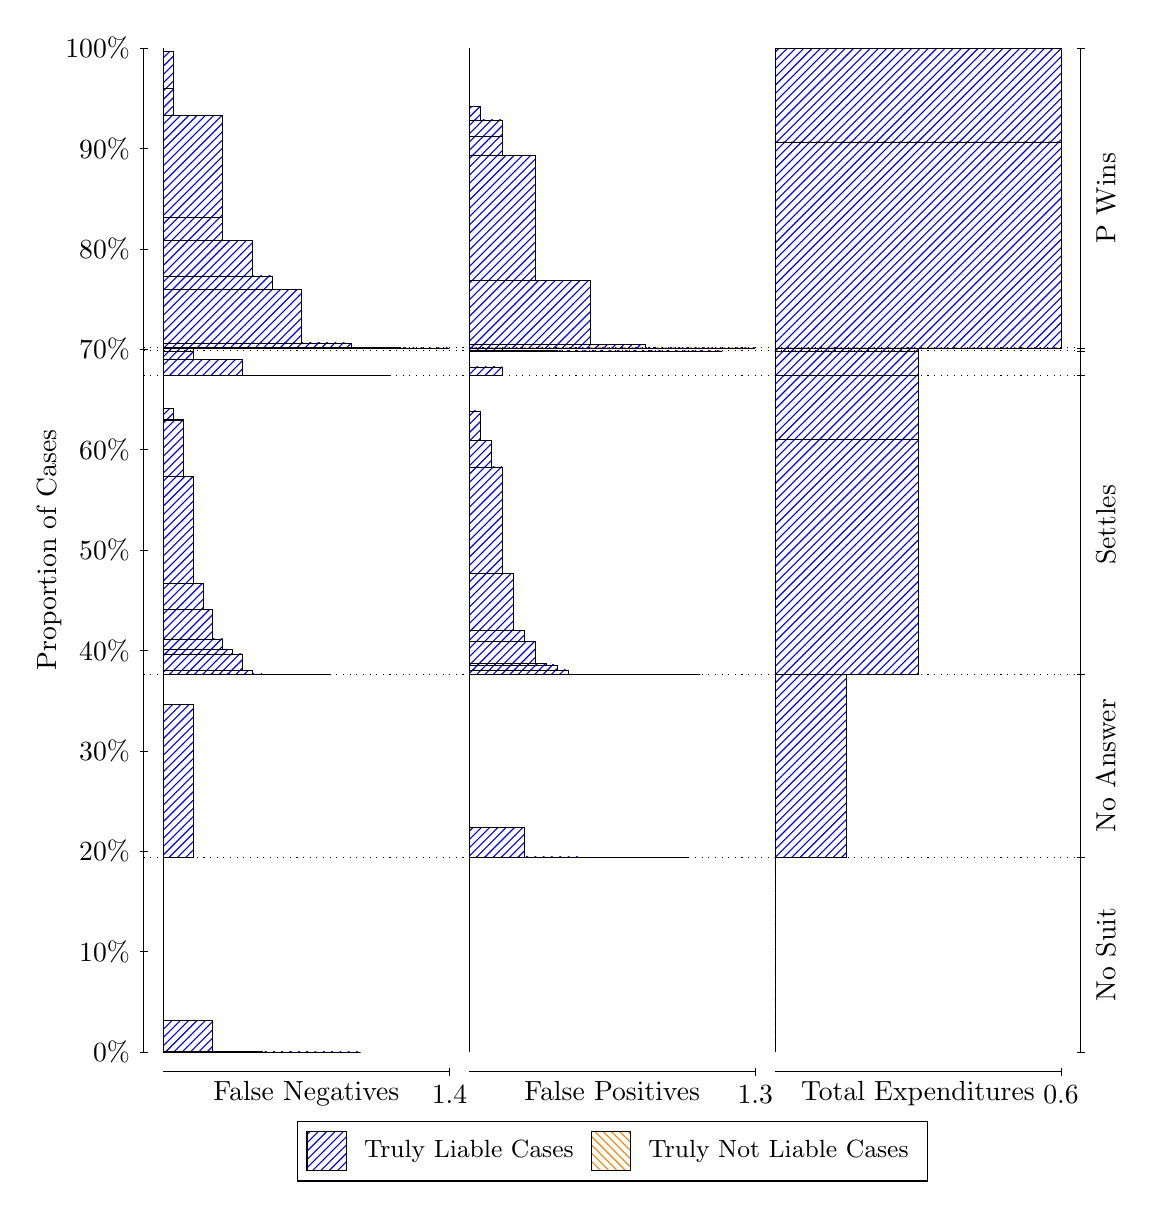
\begin{tikzpicture}
\draw[black, very thin] (1.5,1.75) -- (1.5,14.5);
\node[rotate=90, anchor=center] at (0.3, 8.125) {Proportion of Cases};
\draw[black, very thin] (1.45,1.75) -- (1.55,1.75);
\node[anchor=east] at (1.45, 1.75) {0\%};
\draw[black, very thin] (1.45,3.025) -- (1.55,3.025);
\node[anchor=east] at (1.45, 3.025) {10\%};
\draw[black, very thin] (1.45,4.3) -- (1.55,4.3);
\node[anchor=east] at (1.45, 4.3) {20\%};
\draw[black, very thin] (1.45,5.575) -- (1.55,5.575);
\node[anchor=east] at (1.45, 5.575) {30\%};
\draw[black, very thin] (1.45,6.85) -- (1.55,6.85);
\node[anchor=east] at (1.45, 6.85) {40\%};
\draw[black, very thin] (1.45,8.125) -- (1.55,8.125);
\node[anchor=east] at (1.45, 8.125) {50\%};
\draw[black, very thin] (1.45,9.4) -- (1.55,9.4);
\node[anchor=east] at (1.45, 9.4) {60\%};
\draw[black, very thin] (1.45,10.675) -- (1.55,10.675);
\node[anchor=east] at (1.45, 10.675) {70\%};
\draw[black, very thin] (1.45,11.95) -- (1.55,11.95);
\node[anchor=east] at (1.45, 11.95) {80\%};
\draw[black, very thin] (1.45,13.225) -- (1.55,13.225);
\node[anchor=east] at (1.45, 13.225) {90\%};
\draw[black, very thin] (1.45,14.5) -- (1.55,14.5);
\node[anchor=east] at (1.45, 14.5) {100\%};

\draw[black, very thin] (13.4,1.75) -- (13.4,14.5);
\draw[black, very thin] (13.35,1.75) -- (13.45,1.75);
\node[anchor=west] at (13.35, 1.75) {};
\draw[black, very thin] (13.35,4.2243) -- (13.45,4.2243);
\node[anchor=west] at (13.35, 4.2243) {};
\draw[black, very thin] (13.35,6.5478) -- (13.45,6.5478);
\node[anchor=west] at (13.35, 6.5478) {};
\draw[black, very thin] (13.35,10.339) -- (13.45,10.339);
\node[anchor=west] at (13.35, 10.339) {};
\draw[black, very thin] (13.35,10.654) -- (13.45,10.654);
\node[anchor=west] at (13.35, 10.654) {};
\draw[black, very thin] (13.35,10.693) -- (13.45,10.693);
\node[anchor=west] at (13.35, 10.693) {};
\draw[black, very thin] (13.35,14.5) -- (13.45,14.5);
\node[anchor=west] at (13.35, 14.5) {};

\draw[black, very thin, pattern color=blue, pattern=north east lines] (1.75,1.75) rectangle (4.2557,1.75);
\draw[black, very thin, pattern color=blue, pattern=north east lines] (1.75,1.75) rectangle (3.6293,1.75);
\draw[black, very thin, pattern color=blue, pattern=north east lines] (1.75,1.75) rectangle (3.0029,1.7535);
\draw[black, very thin, pattern color=blue, pattern=north east lines] (1.75,1.7535) rectangle (2.3764,2.1551);
\draw[black, very thin, pattern color=orange, pattern=north west lines] (1.75,2.1551) rectangle (1.75,2.1551);
\draw[black, very thin, pattern color=blue, pattern=north east lines] (1.75,2.1551) rectangle (1.75,4.2243);
\draw[black, very thin, pattern color=blue, pattern=north east lines] (1.75,4.2243) rectangle (2.1259,6.1673);
\draw[black, very thin, pattern color=orange, pattern=north west lines] (1.75,6.1673) rectangle (1.75,6.1673);
\draw[black, very thin, pattern color=blue, pattern=north east lines] (1.75,6.1673) rectangle (1.75,6.5478);
\draw[black, very thin, pattern color=blue, pattern=north east lines] (1.75,6.5478) rectangle (3.8799,6.5478);
\draw[black, very thin, pattern color=blue, pattern=north east lines] (1.75,6.5478) rectangle (3.6293,6.5478);
\draw[black, very thin, pattern color=blue, pattern=north east lines] (1.75,6.5478) rectangle (3.3787,6.5482);
\draw[black, very thin, pattern color=blue, pattern=north east lines] (1.75,6.5482) rectangle (3.2534,6.5482);
\draw[black, very thin, pattern color=blue, pattern=north east lines] (1.75,6.5482) rectangle (3.1282,6.5486);
\draw[black, very thin, pattern color=blue, pattern=north east lines] (1.75,6.5486) rectangle (3.0029,6.5503);
\draw[black, very thin, pattern color=blue, pattern=north east lines] (1.75,6.5503) rectangle (2.8776,6.601);
\draw[black, very thin, pattern color=blue, pattern=north east lines] (1.75,6.601) rectangle (2.7523,6.8045);
\draw[black, very thin, pattern color=blue, pattern=north east lines] (1.75,6.8045) rectangle (2.627,6.8591);
\draw[black, very thin, pattern color=blue, pattern=north east lines] (1.75,6.8591) rectangle (2.5017,6.9954);
\draw[black, very thin, pattern color=blue, pattern=north east lines] (1.75,6.9954) rectangle (2.3764,7.3661);
\draw[black, very thin, pattern color=blue, pattern=north east lines] (1.75,7.3661) rectangle (2.2511,7.7053);
\draw[black, very thin, pattern color=blue, pattern=north east lines] (1.75,7.7053) rectangle (2.1259,9.0633);
\draw[black, very thin, pattern color=blue, pattern=north east lines] (1.75,9.0633) rectangle (2.0006,9.7784);
\draw[black, very thin, pattern color=blue, pattern=north east lines] (1.75,9.7784) rectangle (2.0006,9.7846);
\draw[black, very thin, pattern color=blue, pattern=north east lines] (1.75,9.7846) rectangle (1.8753,9.9201);
\draw[black, very thin, pattern color=orange, pattern=north west lines] (1.75,9.9201) rectangle (1.75,9.9201);
\draw[black, very thin, pattern color=blue, pattern=north east lines] (1.75,9.9201) rectangle (1.75,10.339);
\draw[black, very thin, pattern color=blue, pattern=north east lines] (1.75,10.339) rectangle (4.6316,10.339);
\draw[black, very thin, pattern color=blue, pattern=north east lines] (1.75,10.339) rectangle (4.0052,10.339);
\draw[black, very thin, pattern color=blue, pattern=north east lines] (1.75,10.339) rectangle (3.3787,10.346);
\draw[black, very thin, pattern color=blue, pattern=north east lines] (1.75,10.346) rectangle (2.7523,10.543);
\draw[black, very thin, pattern color=blue, pattern=north east lines] (1.75,10.543) rectangle (2.1259,10.654);
\draw[black, very thin, pattern color=orange, pattern=north west lines] (1.75,10.654) rectangle (1.75,10.654);
\draw[black, very thin, pattern color=blue, pattern=north east lines] (1.75,10.654) rectangle (2.1259,10.687);
\draw[black, very thin, pattern color=orange, pattern=north west lines] (1.75,10.687) rectangle (1.75,10.687);
\draw[black, very thin, pattern color=blue, pattern=north east lines] (1.75,10.687) rectangle (1.75,10.693);
\draw[black, very thin, pattern color=blue, pattern=north east lines] (1.75,10.693) rectangle (5.3833,10.693);
\draw[black, very thin, pattern color=blue, pattern=north east lines] (1.75,10.693) rectangle (4.7569,10.694);
\draw[black, very thin, pattern color=blue, pattern=north east lines] (1.75,10.694) rectangle (4.381,10.694);
\draw[black, very thin, pattern color=blue, pattern=north east lines] (1.75,10.694) rectangle (4.1305,10.756);
\draw[black, very thin, pattern color=blue, pattern=north east lines] (1.75,10.756) rectangle (3.7546,10.756);
\draw[black, very thin, pattern color=blue, pattern=north east lines] (1.75,10.756) rectangle (3.504,11.432);
\draw[black, very thin, pattern color=blue, pattern=north east lines] (1.75,11.432) rectangle (3.1282,11.605);
\draw[black, very thin, pattern color=blue, pattern=north east lines] (1.75,11.605) rectangle (2.8776,12.058);
\draw[black, very thin, pattern color=blue, pattern=north east lines] (1.75,12.058) rectangle (2.5017,12.35);
\draw[black, very thin, pattern color=blue, pattern=north east lines] (1.75,12.35) rectangle (2.5017,13.644);
\draw[black, very thin, pattern color=blue, pattern=north east lines] (1.75,13.644) rectangle (2.2511,13.644);
\draw[black, very thin, pattern color=blue, pattern=north east lines] (1.75,13.644) rectangle (1.8753,13.99);
\draw[black, very thin, pattern color=blue, pattern=north east lines] (1.75,13.99) rectangle (1.8753,14.454);
\draw[black, very thin, pattern color=orange, pattern=north west lines] (1.75,14.454) rectangle (1.75,14.454);
\draw[black, very thin, pattern color=blue, pattern=north east lines] (1.75,14.454) rectangle (1.75,14.5);
\draw[black, very thin, pattern color=orange, pattern=north west lines] (5.6333,1.75) rectangle (5.6333,1.75);
\draw[black, very thin, pattern color=blue, pattern=north east lines] (5.6333,1.75) rectangle (5.6333,4.2243);
\draw[black, very thin, pattern color=orange, pattern=north west lines] (5.6333,4.2243) rectangle (8.4282,4.2243);
\draw[black, very thin, pattern color=blue, pattern=north east lines] (5.6333,4.2243) rectangle (8.4282,4.2243);
\draw[black, very thin, pattern color=blue, pattern=north east lines] (5.6333,4.2243) rectangle (7.7295,4.2243);
\draw[black, very thin, pattern color=blue, pattern=north east lines] (5.6333,4.2243) rectangle (7.0308,4.2275);
\draw[black, very thin, pattern color=blue, pattern=north east lines] (5.6333,4.2275) rectangle (6.3321,4.6047);
\draw[black, very thin, pattern color=blue, pattern=north east lines] (5.6333,4.6047) rectangle (5.6333,6.5478);
\draw[black, very thin, pattern color=orange, pattern=north west lines] (5.6333,6.5478) rectangle (8.5679,6.5478);
\draw[black, very thin, pattern color=blue, pattern=north east lines] (5.6333,6.5478) rectangle (8.5679,6.5478);
\draw[black, very thin, pattern color=orange, pattern=north west lines] (5.6333,6.5478) rectangle (8.2885,6.5478);
\draw[black, very thin, pattern color=blue, pattern=north east lines] (5.6333,6.5478) rectangle (8.2885,6.5478);
\draw[black, very thin, pattern color=orange, pattern=north west lines] (5.6333,6.5478) rectangle (8.009,6.5478);
\draw[black, very thin, pattern color=blue, pattern=north east lines] (5.6333,6.5478) rectangle (8.009,6.5478);
\draw[black, very thin, pattern color=blue, pattern=north east lines] (5.6333,6.5478) rectangle (7.8692,6.5478);
\draw[black, very thin, pattern color=orange, pattern=north west lines] (5.6333,6.5478) rectangle (7.7295,6.5478);
\draw[black, very thin, pattern color=blue, pattern=north east lines] (5.6333,6.5478) rectangle (7.7295,6.5478);
\draw[black, very thin, pattern color=blue, pattern=north east lines] (5.6333,6.5478) rectangle (7.5897,6.5478);
\draw[black, very thin, pattern color=orange, pattern=north west lines] (5.6333,6.5478) rectangle (7.45,6.5478);
\draw[black, very thin, pattern color=blue, pattern=north east lines] (5.6333,6.5478) rectangle (7.45,6.5478);
\draw[black, very thin, pattern color=blue, pattern=north east lines] (5.6333,6.5478) rectangle (7.3103,6.5478);
\draw[black, very thin, pattern color=orange, pattern=north west lines] (5.6333,6.5478) rectangle (7.1705,6.5478);
\draw[black, very thin, pattern color=blue, pattern=north east lines] (5.6333,6.5478) rectangle (7.1705,6.5485);
\draw[black, very thin, pattern color=blue, pattern=north east lines] (5.6333,6.5485) rectangle (7.0308,6.5488);
\draw[black, very thin, pattern color=blue, pattern=north east lines] (5.6333,6.5488) rectangle (6.891,6.5488);
\draw[black, very thin, pattern color=orange, pattern=north west lines] (5.6333,6.5488) rectangle (6.891,6.5488);
\draw[black, very thin, pattern color=blue, pattern=north east lines] (5.6333,6.5488) rectangle (6.891,6.6023);
\draw[black, very thin, pattern color=blue, pattern=north east lines] (5.6333,6.6023) rectangle (6.7513,6.667);
\draw[black, very thin, pattern color=blue, pattern=north east lines] (5.6333,6.667) rectangle (6.6115,6.684);
\draw[black, very thin, pattern color=blue, pattern=north east lines] (5.6333,6.684) rectangle (6.4718,6.967);
\draw[black, very thin, pattern color=blue, pattern=north east lines] (5.6333,6.967) rectangle (6.3321,7.1025);
\draw[black, very thin, pattern color=blue, pattern=north east lines] (5.6333,7.1025) rectangle (6.1923,7.1087);
\draw[black, very thin, pattern color=blue, pattern=north east lines] (5.6333,7.1087) rectangle (6.1923,7.8237);
\draw[black, very thin, pattern color=blue, pattern=north east lines] (5.6333,7.8237) rectangle (6.0526,9.1818);
\draw[black, very thin, pattern color=blue, pattern=north east lines] (5.6333,9.1818) rectangle (5.9128,9.521);
\draw[black, very thin, pattern color=blue, pattern=north east lines] (5.6333,9.521) rectangle (5.7731,9.8917);
\draw[black, very thin, pattern color=blue, pattern=north east lines] (5.6333,9.8917) rectangle (5.6333,10.339);
\draw[black, very thin, pattern color=orange, pattern=north west lines] (5.6333,10.339) rectangle (6.0526,10.339);
\draw[black, very thin, pattern color=blue, pattern=north east lines] (5.6333,10.339) rectangle (6.0526,10.45);
\draw[black, very thin, pattern color=blue, pattern=north east lines] (5.6333,10.45) rectangle (5.6333,10.654);
\draw[black, very thin, pattern color=orange, pattern=north west lines] (5.6333,10.654) rectangle (8.8474,10.654);
\draw[black, very thin, pattern color=blue, pattern=north east lines] (5.6333,10.654) rectangle (8.8474,10.654);
\draw[black, very thin, pattern color=blue, pattern=north east lines] (5.6333,10.654) rectangle (8.1487,10.654);
\draw[black, very thin, pattern color=blue, pattern=north east lines] (5.6333,10.654) rectangle (7.45,10.654);
\draw[black, very thin, pattern color=blue, pattern=north east lines] (5.6333,10.654) rectangle (6.7513,10.66);
\draw[black, very thin, pattern color=blue, pattern=north east lines] (5.6333,10.66) rectangle (6.0526,10.693);
\draw[black, very thin, pattern color=orange, pattern=north west lines] (5.6333,10.693) rectangle (9.2667,10.693);
\draw[black, very thin, pattern color=blue, pattern=north east lines] (5.6333,10.693) rectangle (9.2667,10.693);
\draw[black, very thin, pattern color=orange, pattern=north west lines] (5.6333,10.693) rectangle (8.5679,10.693);
\draw[black, very thin, pattern color=blue, pattern=north east lines] (5.6333,10.693) rectangle (8.5679,10.693);
\draw[black, very thin, pattern color=orange, pattern=north west lines] (5.6333,10.693) rectangle (7.8692,10.693);
\draw[black, very thin, pattern color=blue, pattern=north east lines] (5.6333,10.693) rectangle (7.8692,10.739);
\draw[black, very thin, pattern color=orange, pattern=north west lines] (5.6333,10.739) rectangle (7.45,10.739);
\draw[black, very thin, pattern color=blue, pattern=north east lines] (5.6333,10.739) rectangle (7.45,10.739);
\draw[black, very thin, pattern color=orange, pattern=north west lines] (5.6333,10.739) rectangle (7.1705,10.739);
\draw[black, very thin, pattern color=blue, pattern=north east lines] (5.6333,10.739) rectangle (7.1705,11.549);
\draw[black, very thin, pattern color=orange, pattern=north west lines] (5.6333,11.549) rectangle (6.7513,11.549);
\draw[black, very thin, pattern color=blue, pattern=north east lines] (5.6333,11.549) rectangle (6.7513,11.549);
\draw[black, very thin, pattern color=blue, pattern=north east lines] (5.6333,11.549) rectangle (6.4718,13.134);
\draw[black, very thin, pattern color=blue, pattern=north east lines] (5.6333,13.134) rectangle (6.0526,13.379);
\draw[black, very thin, pattern color=orange, pattern=north west lines] (5.6333,13.379) rectangle (6.0526,13.379);
\draw[black, very thin, pattern color=blue, pattern=north east lines] (5.6333,13.379) rectangle (6.0526,13.588);
\draw[black, very thin, pattern color=blue, pattern=north east lines] (5.6333,13.588) rectangle (5.7731,13.76);
\draw[black, very thin, pattern color=blue, pattern=north east lines] (5.6333,13.76) rectangle (5.6333,14.5);
\draw[black, very thin, pattern color=orange, pattern=north west lines] (9.5167,1.75) rectangle (9.5167,1.75);
\draw[black, very thin, pattern color=blue, pattern=north east lines] (9.5167,1.75) rectangle (9.5167,4.2243);
\draw[black, very thin, pattern color=orange, pattern=north west lines] (9.5167,4.2243) rectangle (10.425,4.2243);
\draw[black, very thin, pattern color=blue, pattern=north east lines] (9.5167,4.2243) rectangle (10.425,6.5478);
\draw[black, very thin, pattern color=orange, pattern=north west lines] (9.5167,6.5478) rectangle (11.333,6.5478);
\draw[black, very thin, pattern color=blue, pattern=north east lines] (9.5167,6.5478) rectangle (11.333,9.5329);
\draw[black, very thin, pattern color=orange, pattern=north west lines] (9.5167,9.5329) rectangle (11.333,9.5329);
\draw[black, very thin, pattern color=blue, pattern=north east lines] (9.5167,9.5329) rectangle (11.333,10.339);
\draw[black, very thin, pattern color=orange, pattern=north west lines] (9.5167,10.339) rectangle (11.333,10.339);
\draw[black, very thin, pattern color=blue, pattern=north east lines] (9.5167,10.339) rectangle (11.333,10.654);
\draw[black, very thin, pattern color=orange, pattern=north west lines] (9.5167,10.654) rectangle (11.333,10.654);
\draw[black, very thin, pattern color=blue, pattern=north east lines] (9.5167,10.654) rectangle (11.333,10.693);
\draw[black, very thin, pattern color=orange, pattern=north west lines] (9.5167,10.693) rectangle (13.15,10.693);
\draw[black, very thin, pattern color=blue, pattern=north east lines] (9.5167,10.693) rectangle (13.15,13.307);
\draw[black, very thin, pattern color=orange, pattern=north west lines] (9.5167,13.307) rectangle (13.15,13.307);
\draw[black, very thin, pattern color=blue, pattern=north east lines] (9.5167,13.307) rectangle (13.15,14.5);
\draw[black, dotted] (1.5,4.2243) -- (13.4,4.2243);
\draw[black, dotted] (1.5,6.5478) -- (13.4,6.5478);
\draw[black, dotted] (1.5,10.339) -- (13.4,10.339);
\draw[black, dotted] (1.5,10.654) -- (13.4,10.654);
\draw[black, dotted] (1.5,10.693) -- (13.4,10.693);
\draw[black, very thin] (1.75,1.5) -- (5.3833,1.5);
\node[anchor=north] at (3.5667, 1.5) {False Negatives};
\draw[black, very thin] (5.3833,1.45) -- (5.3833,1.55);
\node[anchor=north] at (5.3833, 1.45) {1.4};

\draw[black, very thin] (5.6333,1.5) -- (9.2667,1.5);
\node[anchor=north] at (7.45, 1.5) {False Positives};
\draw[black, very thin] (9.2667,1.45) -- (9.2667,1.55);
\node[anchor=north] at (9.2667, 1.45) {1.3};

\draw[black, very thin] (9.5167,1.5) -- (13.15,1.5);
\node[anchor=north] at (11.333, 1.5) {Total Expenditures};
\draw[black, very thin] (13.15,1.45) -- (13.15,1.55);
\node[anchor=north] at (13.15, 1.45) {0.6};

\node[black, centered, rotate=90] at (13.72, 2.9871) {No Suit};
\node[black, centered, rotate=90] at (13.72, 5.386) {No Answer};
\node[black, centered, rotate=90] at (13.72, 8.4435) {Settles};


\node[black, centered, rotate=90] at (13.72, 12.596) {P Wins};

\draw (7.449999999999999,1.5) node[draw=none] (baseCoordinate) {};
\begin{scope}[align=center]
        \matrix[scale=0.5, draw=black, below=0.5cm of baseCoordinate, nodes={draw}, column sep=0.1cm]{
            \node[rectangle, draw, minimum width=0.5cm, minimum height=0.5cm, pattern=north east lines, pattern color=blue] {}; &
            \node[draw=none, font=\small] (B) {Truly Liable Cases}; &
            \node[rectangle, draw, minimum width=0.5cm, minimum height=0.5cm, pattern=north west lines, pattern color=orange] {}; &
            \node[draw=none, font=\small] (B) {Truly Not Liable Cases}; \\
            };
\end{scope}

\end{tikzpicture}
\end{document}